\section{Results and Analysis}
\label{Results}

Provide experiment results: serial \\
Compare serial vs pthreads vs cuda vs theano. \\
Provide graphs for speedup with increasing problem size \\
Analyze speedup with number of threads/cores used \\
Analyze the level of parallelization obtained \\
Analyze performance bottlenecks \\
Do overall analysis and compare obtained results with your expectations\\

As described in previous sections, we compare our implementations with state of the art deep learning library, Theano, in three different parallelizations (Serial/Pthreads/Cuda-C). All experiments are done under the same network structures with MNIST datasets.

\begin{figure}[ht]
%\vskip 0.2in
\begin{center}
\centerline{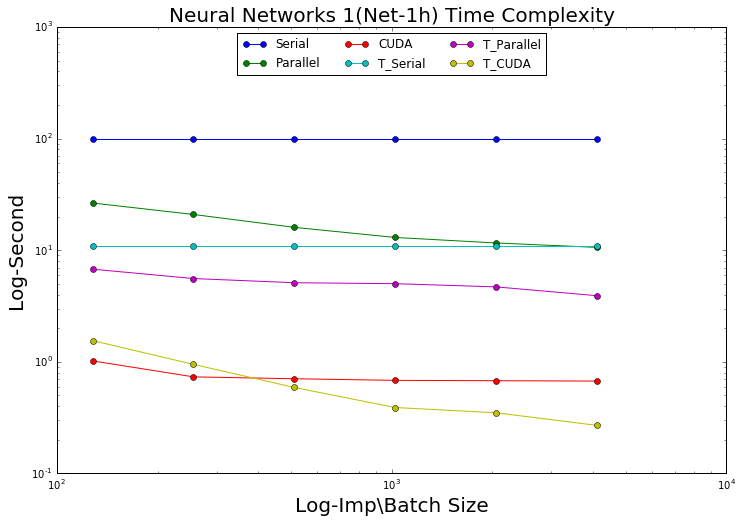
\includegraphics[width=\columnwidth]{../../slide/nn1_time.png}}
\caption{Computation time for Net-1h}
\label{fig:nn1_time}
\end{center}
\vskip -0.4in
\end{figure}

Figure \ref{fig:nn1_time} clearly shows distinct characteristics between serial and parallel computation as well as CPU and GPU based computation. First, the serial learning time (Blue curve, Light blue curve) is almost constant on the varying mini batch size. It is because more batch size means linearly increased computation time in the serial domain. On the other hand, the parallel learning time (Green curve) shows exponentially decreased training time due to multithreads. This behavior is shown commonly in parallel computation based on Theano (T-Parallel). In case of GPU based computation, the overall performance is significantly improved because GPU usually have much more cores than CPU. As a result, \textbf{Why cuda doesn't show exponentially decreased pattern?}.\\
The faster computation by the parallelization is able to be captured by seeing GFLOPS(Giga FLoating point OPerations per Second). Figure \ref{fig:nn1_gflops} shows that parallelization provide much larger number of floating point operations than serial, thus, single core computation.   
\begin{figure}[ht]
%\vskip 0.2in
\begin{center}
\centerline{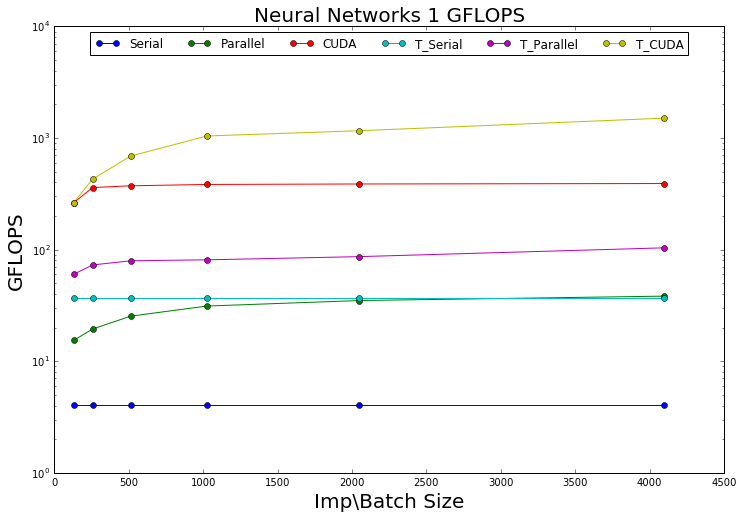
\includegraphics[width=\columnwidth]{../../slide/nn1_gflops.png}}
\caption{GFLOPS for Net-1h}
\label{fig:nn1_gflops}
\end{center}
\vskip -0.4in
\end{figure}



